% R E P O R T E   D E   F R O G G E R
%
% Daniel Ramirez Martinez
% 2 de Nov de 2011
%

\documentclass[letter, 12pt] {article} 

% inclusion de paquetes
\usepackage[spanish] {babel}
\usepackage[utf8] {inputenc}
\usepackage[T1] {fontenc}
\usepackage {sans}   % usa la fuente sans
\usepackage {multicol}  % usa el paquete para multicol
\usepackage {wrapfig}  % se usa para las imagenes con texto alrededor
\usepackage[pdftex] {graphicx}  % para poder usar imagenes


\begin {document}

% pagina de titulo
\begin {titlepage}
  \begin {center}
    % incluye una imagen de 150 px de ancho en la ruta img/Icon.png
    % y despues salta .7 cm
    
\includegraphics[width=150px] {./img/Icon.png} \\[.7cm]
    { \Huge \bfseries Frogger } \\[.4cm]  %titulo en negritas Enorme
    \Large Daniel Ramirez Martinez \\[.2cm]
    \large \today
  \end {center}
\end {titlepage}

% introduccion
\section* {Introducción} % incia una seccion sin numeracion
Implementación mediocre hecha en Java del juego 'Frogger' de Konami 
para Atari 2600. \\[1cm]


\section* {Implementación}  % otra seccion sin numeracion
\subsection* {Mapa} % una subseccion 
El juego consta de un entorno, que a su vez esta compuesto por un
montón de elementos que decienden de la superclase abstracta
'MapElement'.\\

Las secciones (clase 'Section') es una subclase abstracta de 
'MapElement' que determina a los objetos estaticos del entorno.\\

Los actores (clase 'Actors') es una subclase abstracta de 'MapElement'
que determina a los elementos dinamicos del mapa.\\

A continuación se muestra el diagrama de clases.
\begin {center}  %inicia centrado
  % carga una imagen en pdf 
  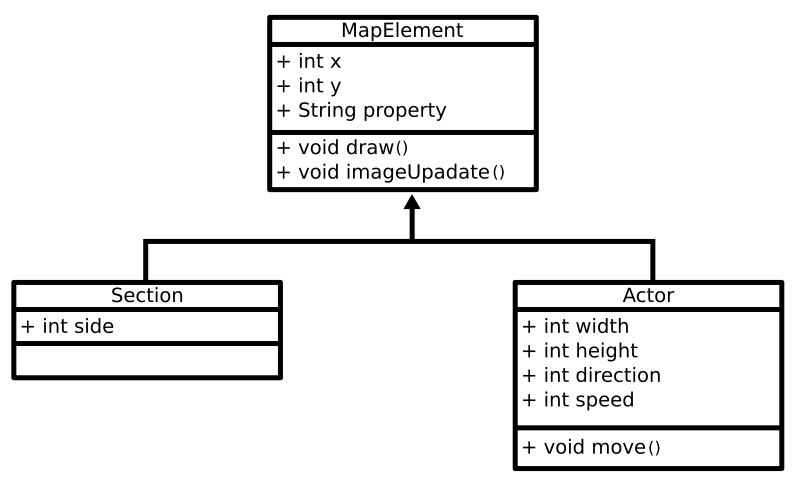
\includegraphics[width=350px]{./img/MapElements-UML.pdf}\\[1cm]
\end {center}

El orden jerarquico de los elementos del entorno esta dado 
en orden ascendente como sigue:

% inicia una lista no ordenada
\begin {itemize}
  \item Terreno
  \item Actores
  \item Jugador
\end {itemize}

% comienza una imagen con texto al rededor
\begin {wrapfigure} {l} {8cm}
  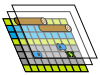
\includegraphics[width=200px]{./img/layer-model.pdf}\\[.5cm]
\end {wrapfigure}

El terreno es un arreglo bidimensional de secciones cuadradas, que
yace bajo las demas capas.\\

Los actores son un arreglo unidimensional de listas, la posición
en el arreglo determina la coordenada en y de el mapa a la que se 
asocia una lista de actores.\\

El jugador simplemente esta sobre todas las demas capas.\\

\subsection* {Detección de colisiones}
La rana es capaz de moverse solo sobre casillas, es decir que siempre
avanzara una casilla completa por lo que la colisión mientras esta 
sobre terreno es muy sencilla ya que solo hay que verificar la 
propiedad de la casilla que le precede al jugador antes de realizar
el movimiento. Por otro caso cuando el jugador esta sobre un actor
el movimiento de la rana ya no es exacto, ya que los actores son
capaces de moverse libremente.\\

\newpage   % salto de pagina

La función de chequeo de colisión en la clase 'Map' verifica si
el arreglo de actores tiene una lista en la posición correspondiente 
a la nueva coordenada 'Y' de la rana. En caso de que si la posea, 
entoces procedera a verificar sobre todos los elementos de dicha lista:
\begin {itemize}
  \item si x esta dentro de K + <alguna tolerancia>\\ 
  \item si x + i esta dentro K - <alguna tolerancia>\\
\end {itemize}

\begin {center}
  \includegraphics[width=200px]{./img/collision.pdf}\\[.5cm]
\end {center}
La función realizara este chequeo para todos los elementos de la
lista a excepción de que en efecto colisione, entonces retornara en
ese elemento con algún código de salida. \\

En caso de que el arreglo de actores no posea una lista en la 
posición correspondiente a la nueva cooredenada 'Y' de la rana, 
entonces retornara inmediatamente con el estado de no colisión
y se verificara el elemento del terreno en la casilla de terreno
correspondiente. \\

Cuando un actor esta sobre otro este adopta su velocidad, por lo
que cuando la rana sube sobre un tronco esta se mueve con el.

\newpage

\subsection* {Juego}
El juego esta regido por un 'Timer' que realiza la acción cada 90
milisegundos.\\

El jugador adquiere: 
\begin {itemize}
  \item 10 puntos: por cada casilla que suba
  \item 100 puntos: por tomar una rana bonus
  \item 200 puntos: por cada rana salvada (que llegue a la meta).
\end {itemize}

Por cada 1000 puntos o cada rana salvada el jugador adquiere mas 
tiempo de juego. \\

Si se acaba el tiempo de juego el jugador pierde una vida. \\

\section* {Problemas}
\subsection* {Sonido}
Culpen a open-jdk-1.6.0\_22, jdk-1.7 y a mis escasos conocimientos
sobre sonido en java (y en todos los lenguajes).

\subsection* {Eventos con el teclado}
no fue posible restringir el abuso en el movimiento de la rana por
parte del usuario.

\subsection* {Gestión de tiempo}
No se pudo implementar un contador para el tiempo de juego basado en
una constante de timepo real. Todo era relativo al 'Timer'.

\end {document} 


